
% ----------------------------------------------------------------------
%  Set the document class
% ----------------------------------------------------------------------
\documentclass[11pt,a4paper,twoside]{article}

% ----------------------------------------------------------------------
% Define external packages, language, margins, fonts and new commands
% ----------------------------------------------------------------------
%\input{preamble} 
\usepackage[utf8]{inputenc}   % <<<<< Linux
\usepackage[english]{babel} % <<<<< English
\usepackage{notoccite}
\usepackage[skip=0.5\baselineskip]{caption}
\hyphenation{GTKWave}
\usepackage{listings}
\usepackage[all]{nowidow}

%blind text
\usepackage{lipsum}

\usepackage{graphicx}
\graphicspath{{./}{../../figlib/}{../mat/}{../sim/}}
\def\FontLn{% 16 pt normal
  \usefont{T1}{phv}{m}{n}\fontsize{16pt}{16pt}\selectfont}
\def\FontLb{% 16 pt bold
  \usefont{T1}{phv}{b}{n}\fontsize{16pt}{16pt}\selectfont}
\def\FontMn{% 14 pt normal
  \usefont{T1}{phv}{m}{n}\fontsize{14pt}{14pt}\selectfont}
\def\FontMb{% 14 pt bold
  \usefont{T1}{phv}{b}{n}\fontsize{14pt}{14pt}\selectfont}
\def\FontSn{% 12 pt normal
  \usefont{T1}{phv}{m}{n}\fontsize{12pt}{12pt}\selectfont}

% Use Arial font as default
%
\renewcommand{\rmdefault}{phv}
\renewcommand{\sfdefault}{phv}
\usepackage{geometry}	
\geometry{verbose,tmargin=2.5cm,bmargin=2.5cm,lmargin=2.5cm,rmargin=2.5cm}

%\usepackage{setspace}
%\renewcommand{\baselinestretch}{1.5}

\usepackage[pdftex]{hyperref} % enhance documents that are to be
                              % output as HTML and PDF
\hypersetup{colorlinks,       % color text of links and anchors,
                              % eliminates borders around links
%            linkcolor=red,    % color for normal internal links
            linkcolor=black,  % color for normal internal links
            anchorcolor=black,% color for anchor text
%            citecolor=green,  % color for bibliographical citations
            citecolor=black,  % color for bibliographical citations
%            filecolor=magenta,% color for URLs which open local files
            filecolor=black,  % color for URLs which open local files
%            menucolor=red,    % color for Acrobat menu items
            menucolor=black,  % color for Acrobat menu items
%            pagecolor=red,    % color for links to other pages
            pagecolor=black,  % color for links to other pages
%            urlcolor=cyan,    % color for linked URLs
            urlcolor=black,   % color for linked URLs
	          bookmarks=true,         % create PDF bookmarks
	          bookmarksopen=false,    % don't expand bookmarks
	          bookmarksnumbered=true, % number bookmarks
	          pdftitle={report},
            pdfauthor={Andre C. Marta},
%            pdfsubject={Thesis Title},
%            pdfkeywords={Thesis Keywords},
            pdfstartview=FitV,
            pdfdisplaydoctitle=true}

\usepackage[numbers,sort&compress]{natbib} % <<<<< References in numbered list [1],[2],...
\usepackage{subcaption} 
\usepackage{mdframed}

%%%%%%%%%%%%%%%%%%%%%%%%%%%%%%%%%%%%%%%%%%%%%%%%%%%%%%%%%%%%%%%%%%%%%%%%
%     Begin Document                                                   %
%%%%%%%%%%%%%%%%%%%%%%%%%%%%%%%%%%%%%%%%%%%%%%%%%%%%%%%%%%%%%%%%%%%%%%%%


\begin{document}

% Set plain page style (no headers, footer with centered page number)
\pagestyle{plain}

% Set roman numbering (i,ii,...) before the start of chapters
%\pagenumbering{roman}

% ----------------------------------------------------------------------
%  Cover page
% ----------------------------------------------------------------------
%%%%%%%%%%%%%%%%%%%%%%%%%%%%%%%%%%%%%%%%%%%%%%%%%%%%%%%%%%%%%%%%%%%%%%%%
%                                                                      %
%     File: Thesis_FrontCover.tex                                      %
%     Tex Master: Thesis.tex                                           %
%                                                                      %
%     Author: Andre C. Marta                                           %
%     Last modified :  2 Jul 2015                                      %
%                                                                      %
%%%%%%%%%%%%%%%%%%%%%%%%%%%%%%%%%%%%%%%%%%%%%%%%%%%%%%%%%%%%%%%%%%%%%%%%

\thispagestyle {empty}

% IST Logo - Signature A
% parameters: bb=llx lly urx ury (bounding box), width=h_length, height=v_length, angle=angle, scale=factor, clip=true/false, draft=true/false. 
\includegraphics[bb=9.5cm 11cm 0cm 0cm,scale=0.29]{IST_A_CMYK_POS}

\begin{center}
%
% Figure (Image or plot)
\vspace{1.0cm}
% height = 50 mm
%\includegraphics[height=50mm]{Figures/Airbus_A350.jpg}

% Title, author and degree
\vspace{1cm}
{\FontLb Circuit Theory and Electronics Fundamentals} \\ % <<<<< EDIT TITLE
\vspace{1cm}
{\FontSn MEAer (Integrated Master In Aerospace Engineering), Técnico, University of Lisbon} \\ % <<<<< EDIT COURSE
\vspace{1cm}
{\FontSn Laboratory 1: Circuit analysis methods} \\
\vspace{1cm}
{\FontSn Group 3} \\
\vspace{0.7cm}
{\FontSn Diogo Faustino, nº95782} \\
\vspace{0.4mm}
{\FontSn Henry Machado, nº95795} \\
\vspace{0.4mm}
{\FontSn Rúben Novais, nº95843} \\
\vspace{1cm}
{\FontSn March 22, 2021} \\ % <<<<< EDIT DATE (corresponds to date of oral examination)
%
\end{center}



% ----------------------------------------------------------------------
% Dedication page (optional)
% ----------------------------------------------------------------------
%\input{dedication} 
%\cleardoublepage

% ----------------------------------------------------------------------
%  Acknowledgments (optional)
% ----------------------------------------------------------------------
%\input{acknowledgements}
%\cleardoublepage

% ----------------------------------------------------------------------
%  Abstract (both in English and Portuguese)
% ----------------------------------------------------------------------
%\input{resumo} 
%\cleardoublepage

%\input{abstract} 

% ----------------------------------------------------------------------
%  Table of contents, list of tables, list of figures and nomenclature
% ----------------------------------------------------------------------

% Table of contents
%
\tableofcontents

% List of tables
%\addcontentsline{toc}{section}{\listtablename}
%\listoftables
%\cleardoublepage 

% List of figures
%\addcontentsline{toc}{section}{\listfigurename}
%\listoffigures
%\cleardoublepage 

% Set arabic numbering (1,2,...) after preface
%
%\setcounter{page}{1}
%\pagenumbering{arabic}

% ----------------------------------------------------------------------
%  Body
% ----------------------------------------------------------------------

\section{Introduction}
\label{sec:introduction}

% state the learning objective 
The objective of this laboratory assignment is to study a circuit containing 4 independent meshes and a total of 11 branches: an independent voltage source $V_A$, an independent current source $I_D$, a dependent current source $I_B$, and a dependent voltage source $V_C$, all connected to 7 resistances (from $R_1$ through to $R_7$). The circuit can be seen in Figure~\ref{fig:rc}.

In Section~\ref{sec:analysis}, a theoretical analysis of the circuit using both the mesh method and the node method is
presented. In Section~\ref{sec:simulation}, the circuit is analysed by
simulation, and the results in operating point are compared to the theoretical results obtained in
Section~\ref{sec:analysis}. The conclusions of this study are laid out in
Section~\ref{sec:conclusion}.

\begin{figure}[h] \centering
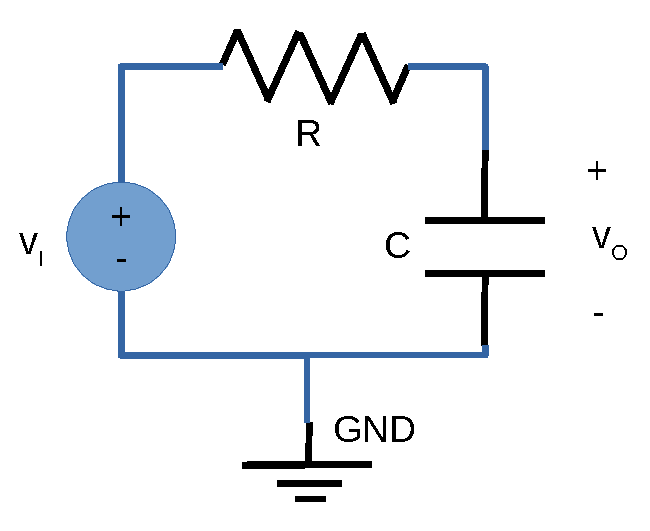
\includegraphics[width=0.9\linewidth]{rc.pdf}
\caption{Circuit with linear components.}
\label{fig:rc}
\end{figure}



\section{Theoretical Analysis}
\label{sec:analysis}

In this section, the circuit shown in Figure~\ref{fig:rc} is analysed
theoretically, using both mesh and node analysis.
Here, we lay out the background information that was essential for the execution of this assignment. Since the circuit at hand is a simple one we only needed the following information (this is all referenced in Horowitz, P; Hill,W(2015). The Art of Electronics. Cambridge University Press(3rd ed, pp.2-4)):
The sum of the currents into a point in a circuit equals the sum of the currents out. Each of these points is referred to as a node. This is also known as Kirchhoff’s current law (KCL).
The sum of the voltage drops around any closed circuit is zero.This is Kirchhoff’s voltage law (KVL).
The power consumed by a circuit device is
\begin{equation}
  P=VI;
\end{equation}

When voltages and currents are in the same direction they produce a positive power (the component is consuming energy). Voltages and currents in opposite direction produce negative power (the component is giving forth energy to the circuit)
A resistor is characterized by its resistance:
\begin{equation}
  R=\frac {V}{I};
\end{equation}
This is known as Ohm’s law.
Independent V/I sources impose voltage/current regardless of current/voltage.
Linearly dependent V/I sources impose voltage/current that is linearly dependent on a specific variable of other circuit component.

The circuit consists of four independent meshes, and 11 branches where different currents circulate. These will be our variables in the mesh analysis. The current flow is depicted in Figure ~\ref{fig:current}


The components we are working with have a linear relationship between the voltage and current, therefore we will need to solve a system of linear equations to determine the variables of each component given some initial values.
We will use two different methods that are based on KCL and KVL. These methods are the Mesh and Node methods. Each one of them will produce its set of equations that when solved, will give  us either the currents flowing through each mesh (Mesh Method) or the voltage on each node (Node Method).
We’ve written a program on GNU Octave to help us determine the solution for the linear system. The simulation of the circuit was carried out by the Ngspice tool. We’ve written a simple code describing the circuit.

\begin{figure}[h] \centering
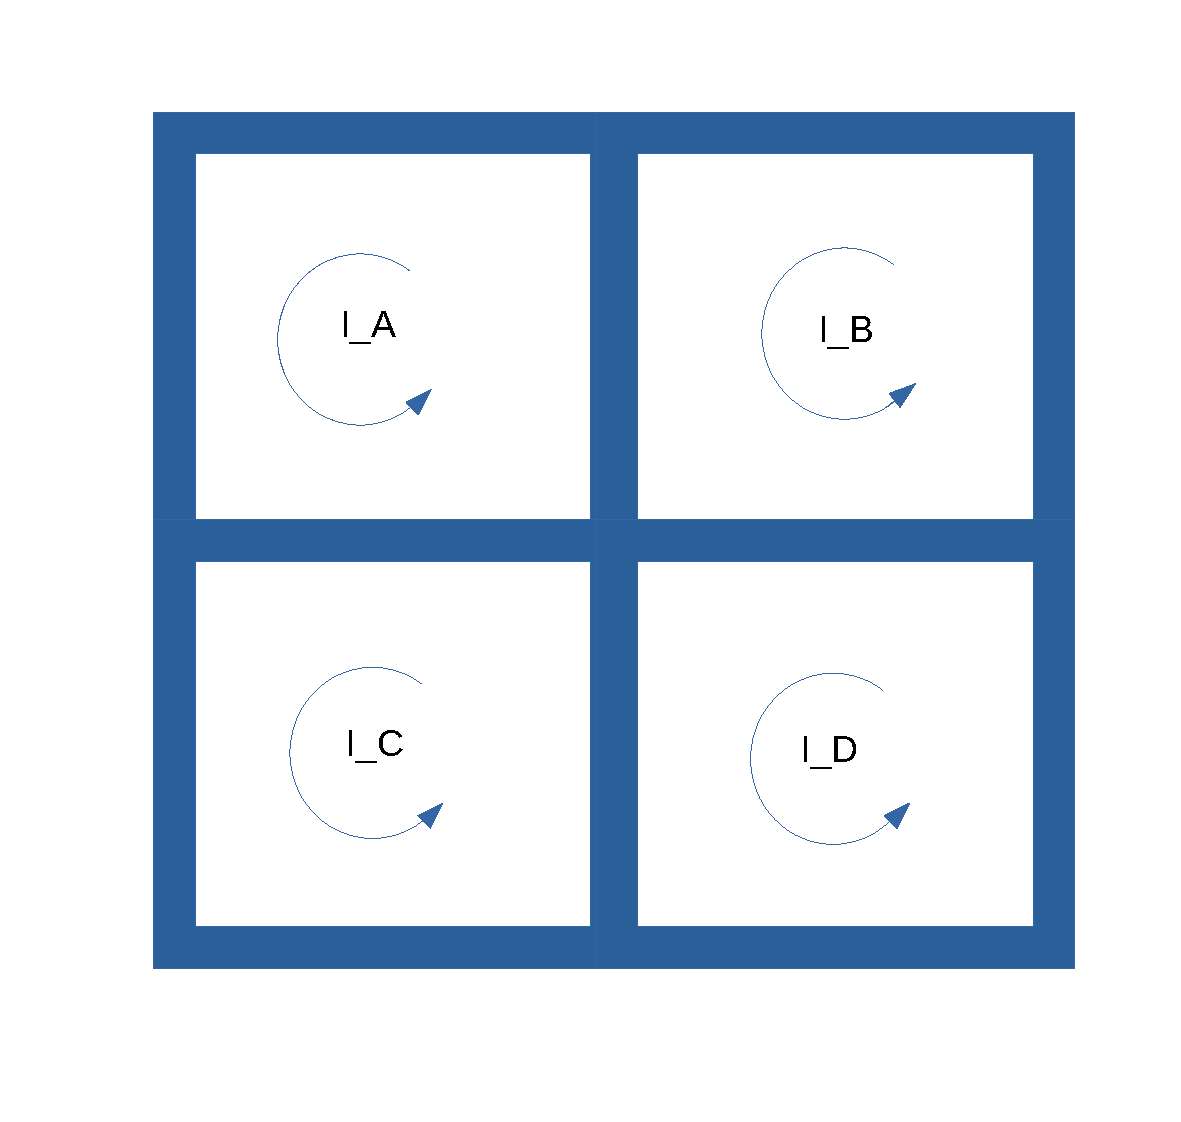
\includegraphics[width=0.4\linewidth]{current.pdf}
\caption{Direction of each mesh current.}
\label{fig:current}
\end{figure}

\subsection{Mesh Analysis}


Applying the Kirchhoff Voltage Law (KVL) in the different loops, we get four different equations, which we can then solve as a matrix:
\begin{equation}
  I_D=I;
\end{equation}

\begin{equation}
  (R_1+R_3+R_4)I_A-R_3I_B-R_4I_C=-V_A;
\end{equation}

\begin{equation}
  (R_4+R_6+R_7-K_C)I_C-R_4I_A=0;
\end{equation}

\begin{equation}
  (R_3K_B-1)I_B-R_3K_BI_A=0.
\end{equation}

\begin{equation}
\begin{pmatrix}
0 & 0 & 0 & 1 \\
R1+R3+R4 & -R3 & -R4 & 0 \\
-R4 & 0 & R4+R6+R7-Kc & 0 \\
-R3Kb & R3Kb-1 & 0 & 0
\end{pmatrix}
\begin{pmatrix}
Ia\\
Ib\\
Ic\\
Id
\end{pmatrix}
=
\begin{pmatrix}
I\\
-V\\
0\\
0
\end{pmatrix}
\end{equation}



\begin{table}[h]
  \centering
  \begin{tabular}{|l|r|}
    \hline    
    {\bf Name} & {\bf Value [A]} \\ \hline
    \input{data_current_tab} 
  \end{tabular}
  \caption{Theoretical analysis results from Octave. (A variable preceded by @ is of type {\em current})}
  \label{tab:mesh}
\end{table}

\subsection{Node Analysis}

As in the previous section, we extract a set of equations from the circuit, this time using the node method. This yields 8 equations, one for each node. Then, we can solve those 8 equations in the form of the matrix presented here.
\begin{equation}
\begin{pmatrix}
G7 & 0 & 0 & 0 & 0 & 0 & G6 & 0\\
1 & -1 & 0 & 0 & 0 & 0 & 0 & 0\\
0 & 0 & 0 & 0 & 0 & 1 & -1 & 0\\
0 & 0 & 0 & -G2 & G1+G2+G3 & -G1 & 0 & -G3\\
0 & 0 & G5 & 0 & G3 & 0 & G4+G6 & -G3-G4-G5\\
1 & 0 & 0 & 0 & 0 & 0& Kc*G6 & -1\\
0 & 0 & 0 & 0 & G1 & -G1 & -G4-G6 & G4\\
0 & 0 & 0 & -G2 & Kb+G2 & 0 & 0 & -Kb
\end{pmatrix}
\begin{pmatrix}
V1\\
V2\\
V3\\
V4\\
V5\\
V6\\
V7\\
V8
\end{pmatrix}
=
\begin{pmatrix}
0\\
0\\
V\\
0\\
I\\
0\\
0\\
0
\end{pmatrix}
\end{equation}

\begin{table}[h]
  \centering
  \begin{tabular}{|l|r|}
    \hline    
    {\bf Name} & {\bf Value [V]} \\ \hline
    \input{data_voltage_tab} 
  \end{tabular}
  \caption{Theoretical analysis results from Octave.}
  \label{tab:node}
\end{table}


\section{Simulation Analysis}
\label{sec:simulation}

\subsection{Operating Point Analysis}

Table~\ref{tab:op} shows the simulated operating point results for the circuit
under analysis. Compared to the theoretical analysis results, one notices the
following differences: describe and explain the differences.

\begin{table}[h]
  \centering
  \begin{tabular}{|l|r|}
    \hline    
    {\bf Name} & {\bf Value [A or V]} \\ \hline
    @cb[i] & 0.000000e+00\\ \hline
@ce[i] & 0.000000e+00\\ \hline
@q1[ib] & 7.022567e-05\\ \hline
@q1[ic] & 1.404513e-02\\ \hline
@q1[ie] & -1.41154e-02\\ \hline
@q1[is] & 5.765392e-12\\ \hline
@rc[i] & 1.411536e-02\\ \hline
@re[i] & 1.411536e-02\\ \hline
@rf[i] & 7.022567e-05\\ \hline
@rs[i] & 0.000000e+00\\ \hline
v(1) & 0.000000e+00\\ \hline
v(2) & 0.000000e+00\\ \hline
base & 2.254108e+00\\ \hline
coll & 5.765392e+00\\ \hline
emit & 1.411536e+00\\ \hline
vcc & 1.000000e+01\\ \hline

  \end{tabular}
  \caption{Operating point. A variable preceded by @ is of type {\em current}
    and expressed in Ampere; other variables are of type {\it voltage} and expressed in
    Volt.}
  \label{tab:op}
\end{table}

\lipsum[1-1]


\subsection{Transient Analysis}

Figure~\ref{fig:trans} shows the simulated transient analysis results for the
circuit under analysis. Compared to the theoretical analysis results, one
notices the following differences: describe and explain the differences.

\begin{figure}[h] \centering
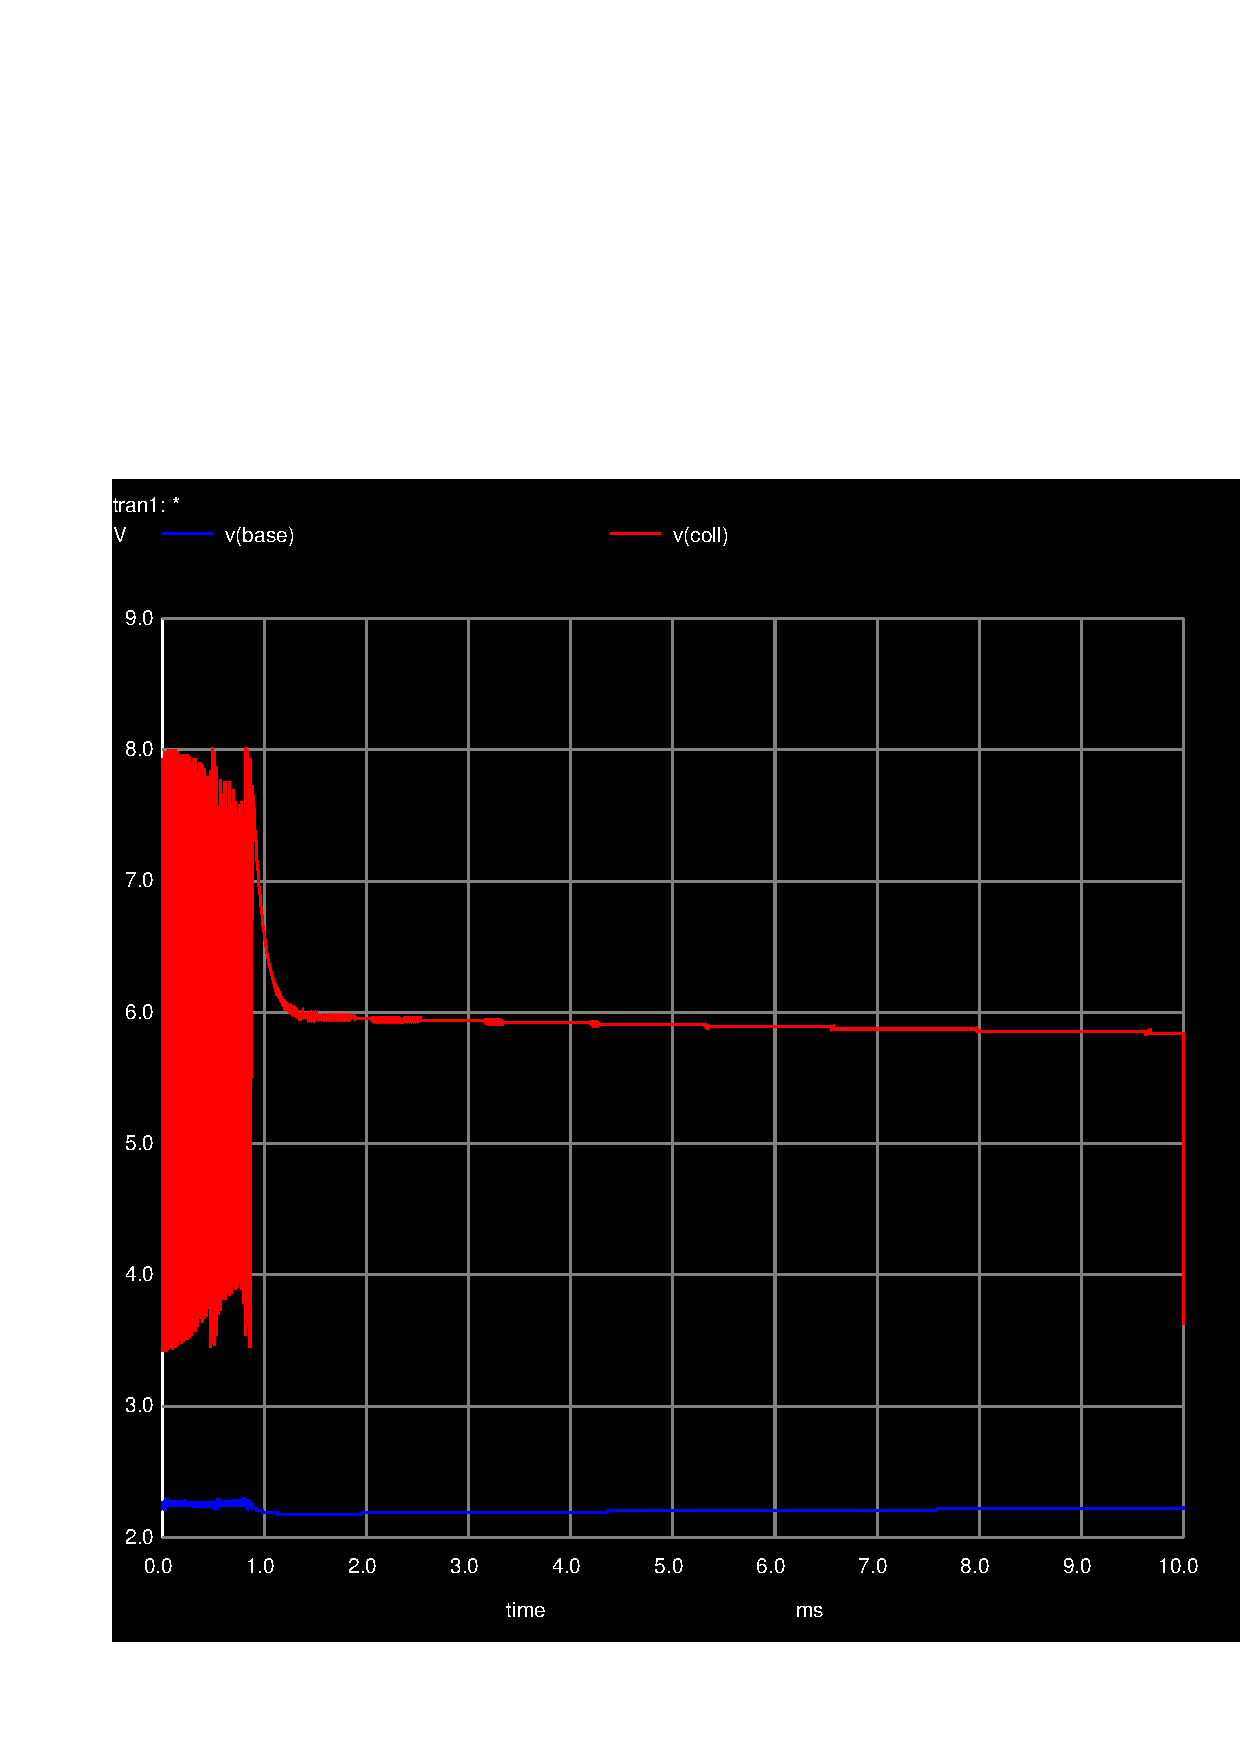
\includegraphics[width=0.6\linewidth]{trans.pdf}
\caption{Transient output voltage}
\label{fig:trans}
\end{figure}

\lipsum[1-1]



\subsection{Frequency Analysis}

\subsubsection{Magnitude Response}

Figure~\ref{fig:acm} shows the magnitude of the frequency response for the
circuit under analysis. Compared to the theoretical analysis results, one
notices the following differences: describe and explain the differences.

\begin{figure}[h] \centering
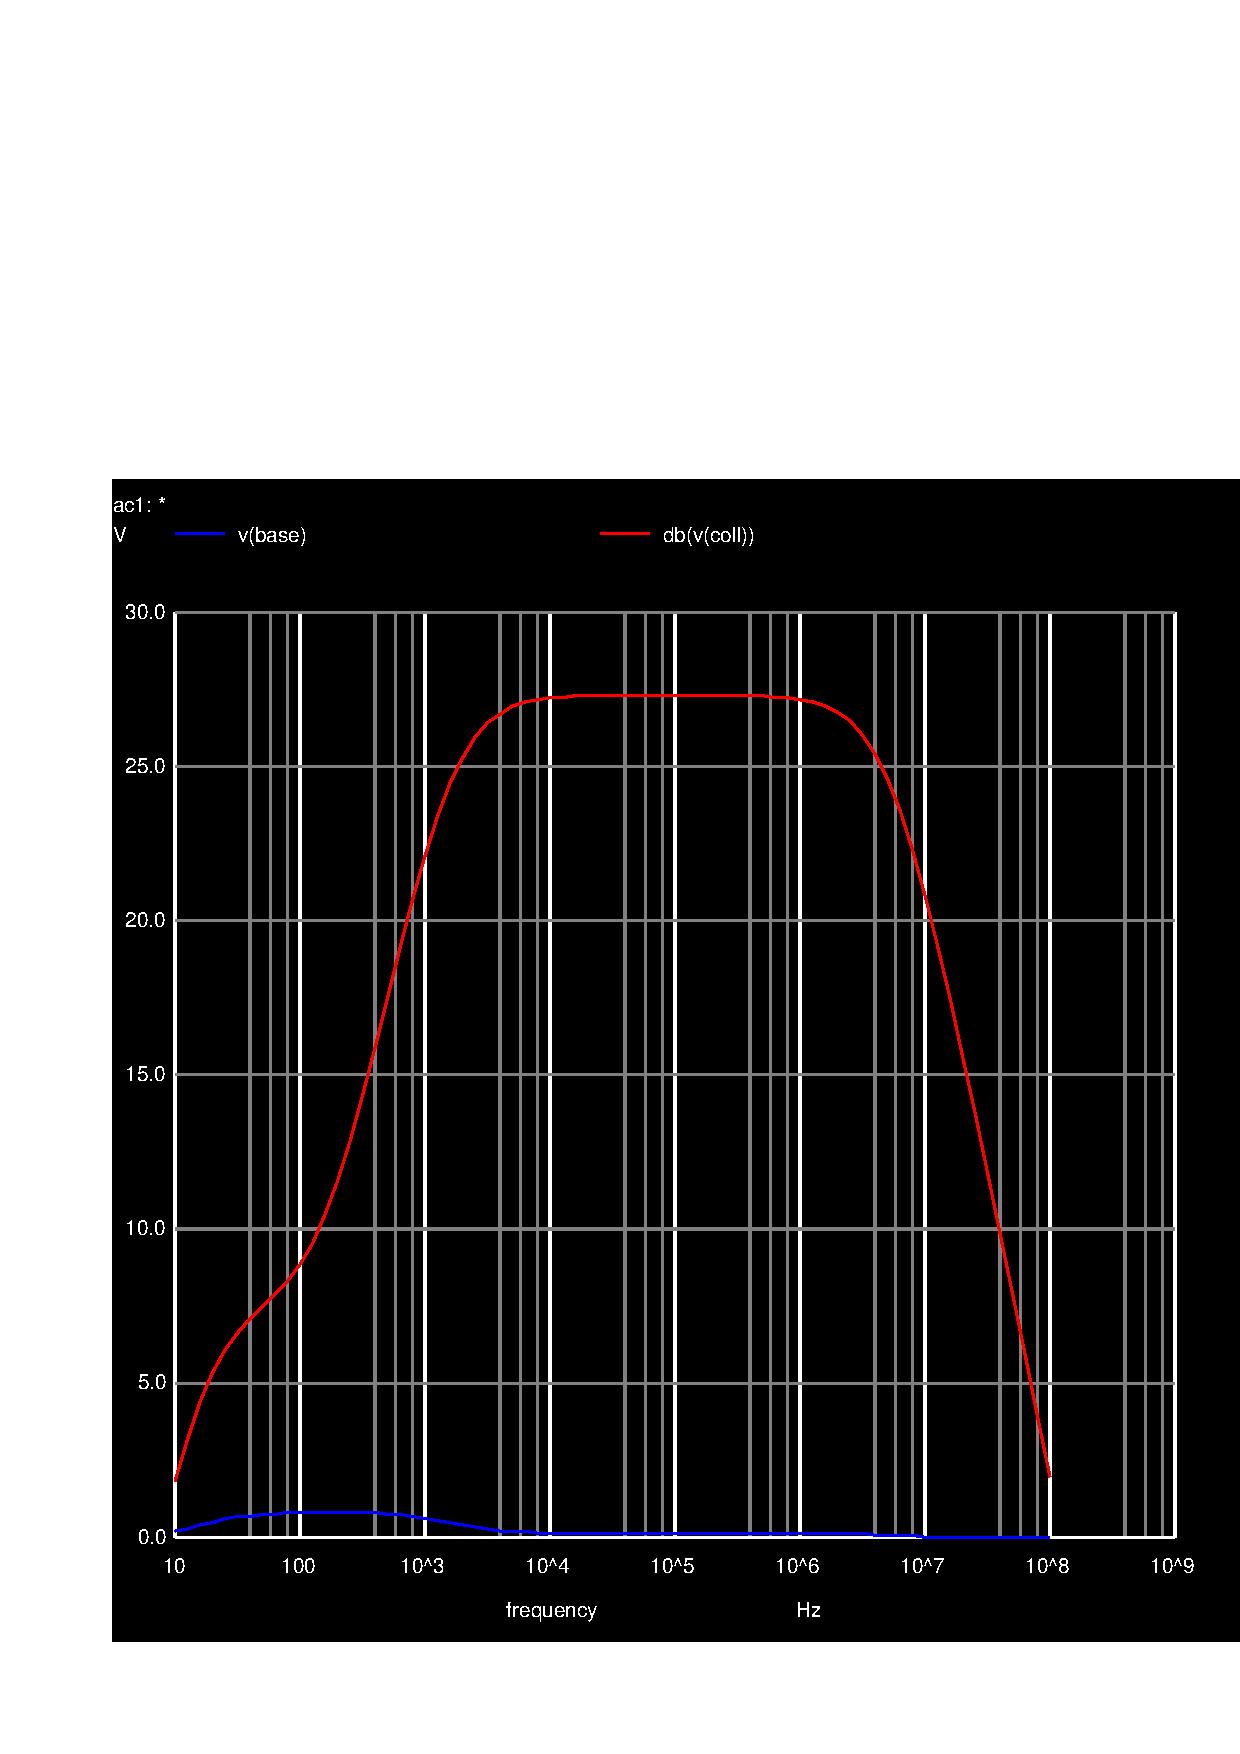
\includegraphics[width=0.6\linewidth]{acm.pdf}
\caption{Magnitude response}
\label{fig:acm}
\end{figure}

\lipsum[1-1]

\subsubsection{Phase Response}

Figure~\ref{fig:acp} shows the magnitude of the frequency response for the
circuit under analysis. Compared to the theoretical analysis results, one
notices the following differences: describe and explain the differences.

\begin{figure}[h] \centering
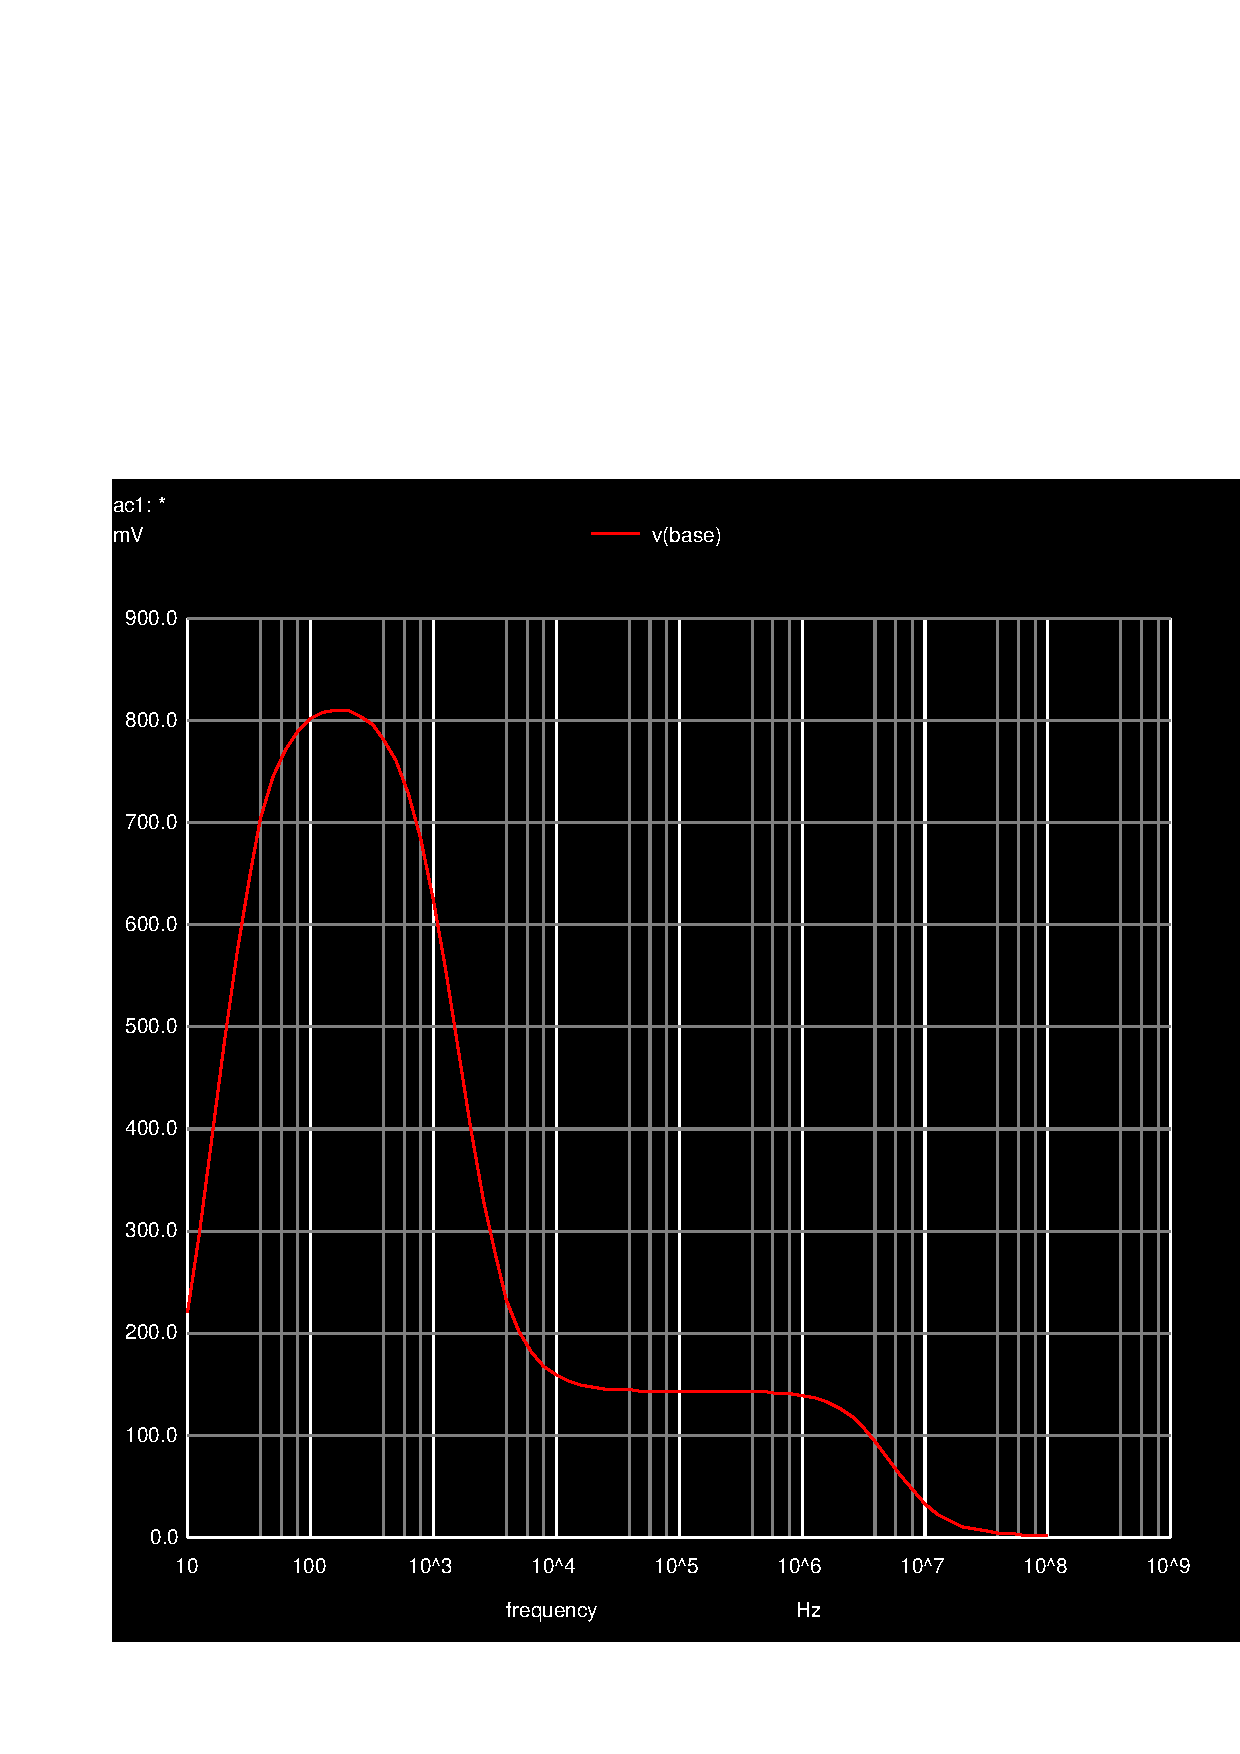
\includegraphics[width=0.6\linewidth]{acp.pdf}
\caption{Phase response}
\label{fig:acp}
\end{figure}

\lipsum[1-1]

\subsubsection{Input Impedance}

Figure~\ref{fig:zim} shows the magnitude of the frequency response for the
circuit under analysis. Compared to the theoretical analysis results, one
notices the following differences: describe and explain the differences.

\begin{figure}[h] \centering
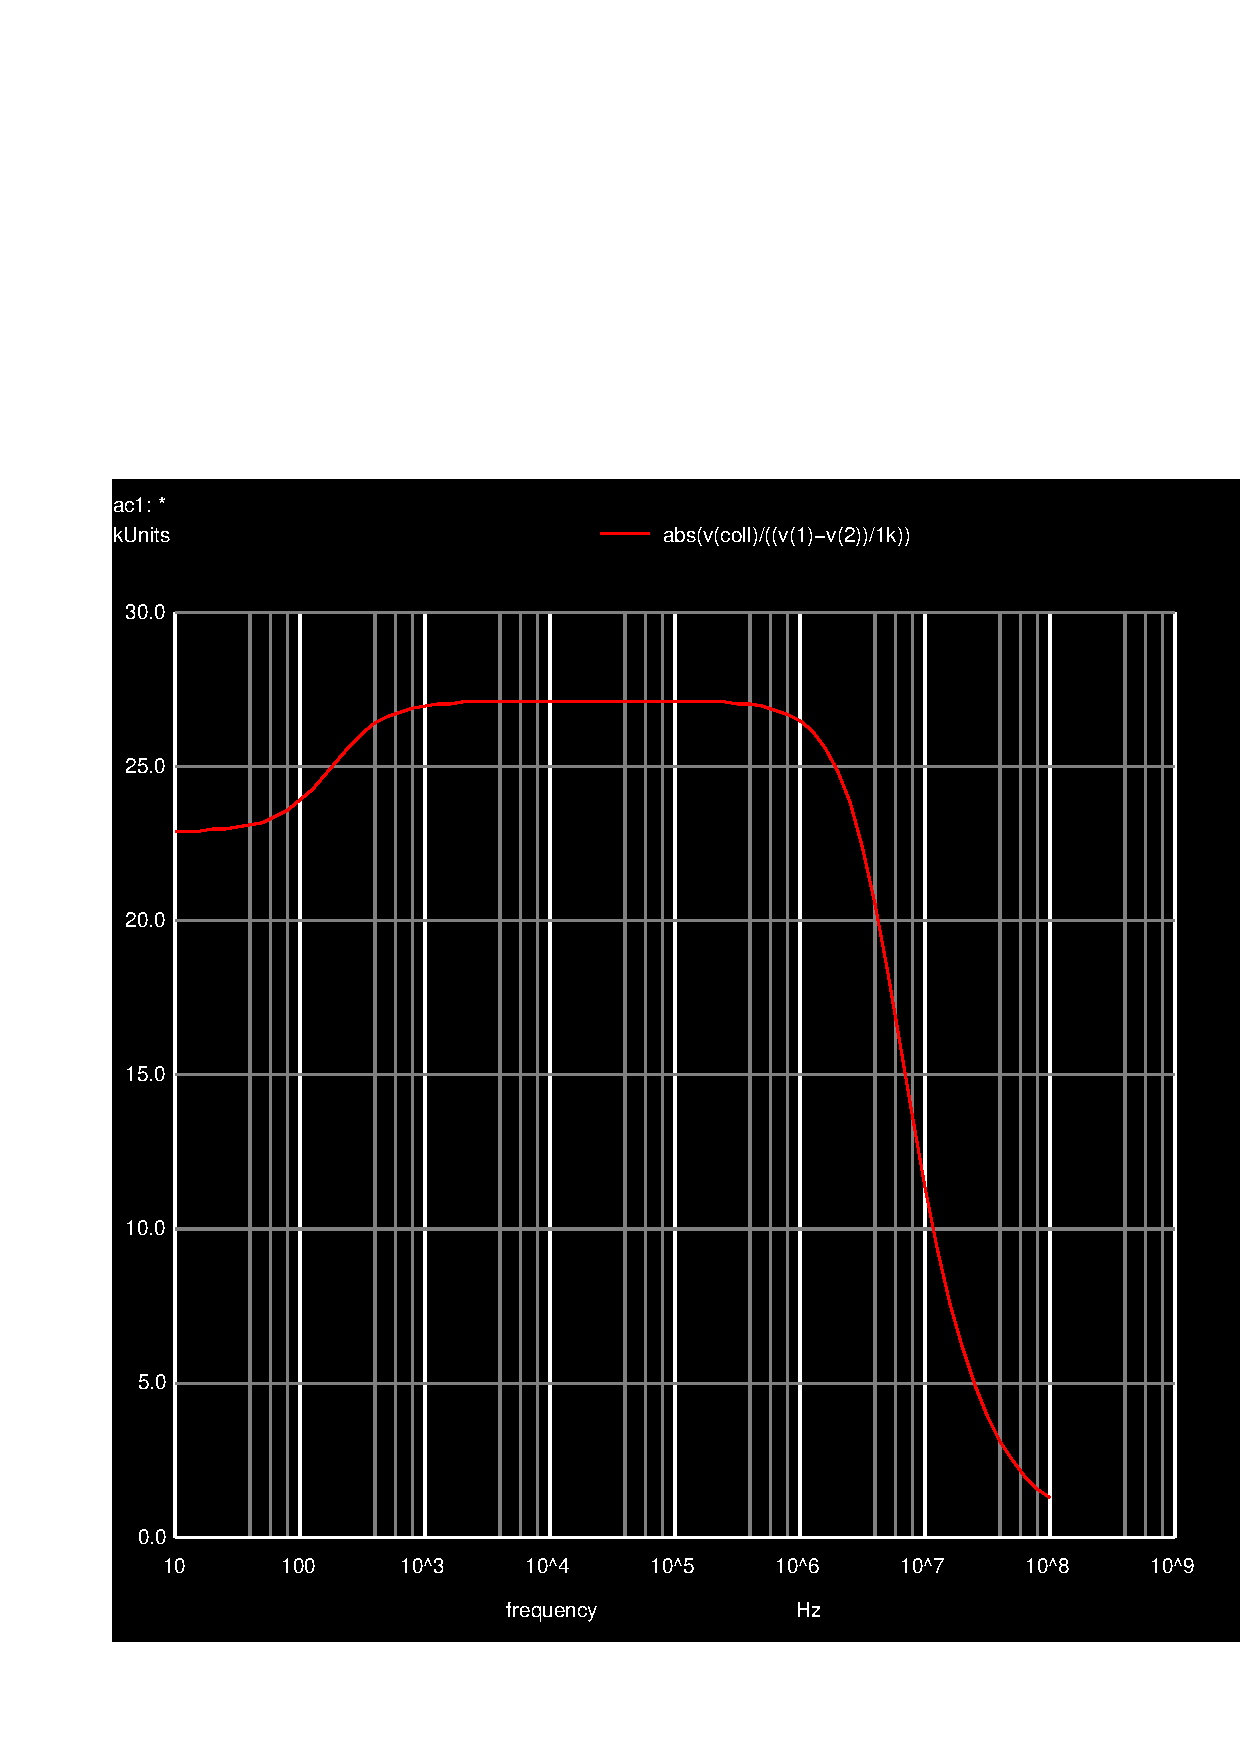
\includegraphics[width=0.6\linewidth]{zim.pdf}
\caption{Input impedance}
\label{fig:zim}
\end{figure}

\lipsum[1-1]





\section{Conclusion}
\label{sec:conclusion}

In this laboratory assignment the objective of analysing an RC circuit has been
achieved. Static, time and frequency analyses have been performed both
theoretically using the Octave maths tool and by circuit simulation using the
Ngspice tool. The simulation results matched the theoretical results
precisely. The reason for this perfect match is the fact that this is a
straightforward circuit containing only linear components, so the theoretical
and simulation models cannot differ. For more complex components, the
theoretical and simulation models could differ but this is not the case in this
work.

\lipsum[1-1]

%\cleardoublepage

% ----------------------------------------------------------------------
%  Bibliography
% ----------------------------------------------------------------------
%\addcontentsline{toc}{section}{\bibname}
%\bibliographystyle{abbrvunsrtnat} % <<<<< SELECT IF USING REFERENCES BY NUMBER (CITATION ORDER)
%\bibliography{../../../BIBfile.bib}

% ----------------------------------------------------------------------
\end{document}
% ----------------------------------------------------------------------
